\chapter{N-Burst Model for LTE Networks}

After many years of research it has become clear that usual models of queuing theory are not sufficient for the modelling many telecommunication services. Maybe one of the reasons for this is that data is not transmitted continuously rather it is transmitted in bursts of packets.But this is not at all enough for explaining the unpredictable performance of routers. This traffic must also be self similar along with bursty. The  self-similar property can be explained and modeled by using power-tailed distributions of burst-sizes.

\section{Some Key Words}
\subsection{Telecommunication Network}
Group of nodes which are joined by links which are used to exchange messages between them. To exchange messages, these links may use packet switching, circuit switching, and many other methods.

\subsection{Self Similarity}
The bursty traffic can be described using the notion of Self-Similarity. This property is often used to describe the infinite complex patterns. However in our case ,this term is used to describe the distribution of object i.e. The distribution of object remains similar even if it is viewed at varying scales.

\subsection{Reliability Function}
It is also called Complementary cumulative distribution function. If we have a non negative variable Z  having mean E(Z). Then it can be described as
\begin{equation}
R_{Z}(x) = Pr(Z > x)
\end{equation}

\subsection{Bursts}
Burst is a group of consecutive packets which have shorter inter-packet gaps than the packets which arrive after or before the burst of packets.

\subsection{Packet Delay}
Time taken by packets to move from source to destination, or rather from one source to another.

\subsection{Buffer Overflow}
When unexpected number of entities arrive at the router the requests are lost, this is called buffer overflow.

\subsection{Semi Markov process}
If we have a process that can be in N states 1,2...N and the system stays in $i^{th}$ state for a random interval of time having mean $\mu_{i}$ and makes a transition to state j with a probability $P_{ij}$ then such a process is called semi-Markov process. Also abbreviated as SM. 

\subsection{Power tail distribution}
Power-Tail distributions with exponent $\beta$ follow the properties
\[
E[X^{l}]= \int_{0}^{\infty} x^{l} f(x) \,dx \begin{cases}
=\infty &\text{for $l\geq \beta$}\\
<\infty &\text{for $l<\beta$}
\end{cases}
\]

Similarly,
\[ 
\lim_{x\to\infty} x^{l}R(x) = \begin{cases}
=\infty \text{ for $l>\beta$}\\
=0 \text{ for $l<\beta$}\\
\end{cases}
\]
\\Density function $c/x^{\beta}$ \text {is a simple form having the above property.}

Truncated Power-Tail distribution is when $x^{\beta}R(x)$ remains almost a constant for large order of magnitudes and drops to 0 eventually\\
\begin{figure}[ht!]
        \centering
        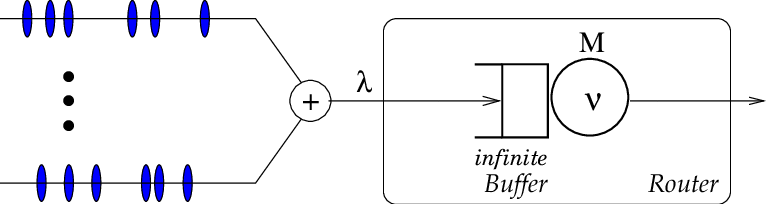
\includegraphics[scale=0.50]{NBurst.png}
        \emph{In this figure the packet generated by each user arrive at a single queue which is maintained by a single router or server }
        \caption{NBurst/M/1 queue}
\end{figure}


\section{LTE Network model}
A simple LTE network consists of a evolved nodeB, which provides service to a set of N wireless devices. 
These devices use the LTE technology for downloading data (down-link) and  upload and request data (up-link).
The mobile devices use several applications to access information using down-link.This results in variable traffic for requests in the LTE system.
Down-link communication will be our main focus.
\\The number of packets requested by a mobile device is considered as a random variable.
The properties and distribution of this random variable is purely based on the mobile application used to request the data.
Which is why standard queuing models are not appropriate to understand telecommunication systems.\\
\begin{figure}[ht!]
        \centering
        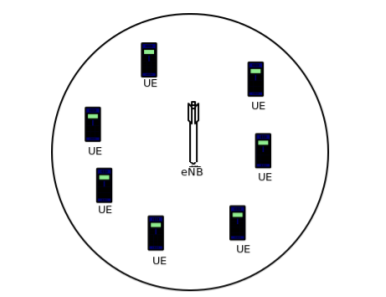
\includegraphics[scale=1]{network.png}
        \\\caption{LTE network topology}
        \label{topology}
\end{figure}

\subsection{Requirements for an appropriate network model}
The main difference from the standard models is the requests in telecommunication networks come in bursts rather than continuously.
The unpredictable traffic must be both bursty and self-similar.
The self similarity can be achieved if the burst sizes are made to follow power-tailed distribution which makes bursts differ in orders of magnitude.

A model settling for  self similarity and burstiness for analysis purpose is not easy. Many models like  M/G/1 queue with changing parameters, batch-arrival model, continuous burst flow models failed to mimic the traffic in telecommunication networks.
A novel queue model N-burst/M/1 is introduced for this purpose.
Independent entities each send forth bursts of packets to a queue on an ON-OFF fashion(bursty model).

\begin{figure}[ht!]
        \centering
        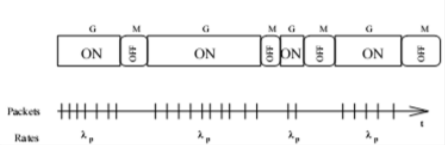
\includegraphics[scale=1]{on-off.PNG}
        \\\caption{On-OFF queue model}
        \label{on-off}
\end{figure}
\section{Description of Model}

N Burst Model is one of the variants of ON-OFF models. The arrival process of N-Burst is the superposition of N ON-OFF type identical and independently distributed source’s traffic streams.
Let (${\lambda}_p$) be the peak transmission rate during a burst i.e. at ON time. No packets are transmitted during OFF period.\\

Given below are the essential parameters of the model :-\\

 \begin{tabular}{rl}
$\kappa$ &:  average rate of packet arrival for each source.\\
$\lambda$ &: The overall arrival rate that is produced by N sources i.e. $\lambda$ =  ${\kappa}N$\\
$N_{b}$ &: Average number of packets during a burst (at ON period)\\
${\lambda}_p$ &:  The peak transmission rate of a node sending packets during a burst. \\
${\lambda}_b$ &: Mean burst arrival rate = $\lambda/N_{b}$\\
$\overline{ON}$ &: the average time during which the node is active\\
$\overline{OFF}$ &: the average time during which the node transmission is OFF.\\
$\mu$ & : the mean service rate of the router\\
$\rho = \frac{\lambda}{\mu}$ &: Load utilisation of the router \\
 \end{tabular}


We have another parameter which is of prime importance called burstiness parameter b defined below:\\

\begin{equation}
b = \frac{\overline{OFF}}{\overline{ON} + \overline{OFF}} = 1 - \frac{\kappa}{{\lambda}_p} = \frac{\lambda}{N{\lambda}_p}\\
\end{equation}
Since $\rho$ (the amount of data sent per unit time), and $\rho$ can be held constant as b is varied over 0 to 1. So the parameter b can be considered as a shape parameter.

\textbf{Case 1}: b=0 \\
When b=0, it means that average time during which the node transmission is OFF is 0. In this case all the bursts come after one another and ON/OFF process reduces to a simple one.\\

\textbf{Case 2}: b=1\\
In this case, the average time during which burst comes is zero. It also means that all the packets in the burst arrive simultaneously i.e. They arrive as a bulk process.\\ 

All other cases of b are not simple and require a careful analysis.\\

\section{Distribution of Sub Processes}

For simplicity let us consider N=1 i.e 1-Burst model.\\
This model depends on four separate distributions , with random variables denoted by $X_{ON}$, $X_{OFF}$, $X_{SV}$ and $X_{INP}$.\\
ON: \textbf{On time distribution} have mean $\overline{ON}$. Therefore the mean number of packets during a burst is given by $N_{b} =  \overline{ON}.\lambda_{p}$  \\
OFF: \textbf{OFF time distribution} have mean $\overline{OFF}$ (It will depend on how often the bursts are generated) \\
SV: \textbf{Service time distribution} has mean 1/$\mu$ ( It will depend on distribution of packet sizes, service rate $\mu$ depends on packet size and router speed)\\
INP: \textbf{Inter packet time distribution} is the distribution during a burst whose mean is 1/$\lambda_{p}$ \\

The parameters to be varied must have to be selected carefully in order to have comparison study of the model useful. We can have two distributions whose means are different but have same shape, whose higher moments will be scaled proportionately. The description of this can be given as:\\
Let X and E(X) be the random variable and its mean respectively, then its Complementary Cumulative Distributive Function be given by\\
\begin{equation}
	R_X{(x)} = Probability(X > x)
\end{equation}

Let Z is the non negative random variable with mean E(Z) and let its distribution has same shape as $R_X(.)$.Then, \\
\[R_Z{(x)} = R_X{(rx)}\text{, where }  r = E(X)/E(Z)\text{, for}\]
\begin{align*}
 E(Z) &=\int_{0}^{\infty} R_Z{(x)} dx\\
 &= \int_{0}^{\infty} R_X{(rx)} dx\\
 &= \int_{0}^{\infty} R_Z{(u)} du/r\\
 &= E(X)/r\\
 &= E(Z) 
\end{align*}
\begin{remark}
Moments of functions which have same shape scale according to the below formula:
\begin{equation}
E(Z^n) = r^nE(X^n)
\end{equation}
or
\begin{equation}
\frac{E(Z^n)}{[E(Z)]^n} = \frac{E(X^n)}{[E(X)]^n}
\end{equation}
\end{remark}

Using this we can vary the distributions of all the above methods and keeping their shapes same.\\

\section{Limiting cases for $b\rightarrow 0$ and $b\rightarrow 1$}
We consider this for 1-Burst process i.e. for N=1.\\
From (2.2) we can conclude that the the transmission of packets can occur at the slowest rate at $\overline{ON}$ times when $\overline{OFF} = 0$ or thus b=0 ($\lambda_{p} = \kappa$). In this case the distribution of $\overline{OFF}$ time is irrelevant.\\
It can be said that since there is no halt in between two bursts , $\overline{ON}$ distribution also does not have an impact on the system.
\begin{remark}
Let $G_{INP}$ represents a general distribution which have Inter arrival times as governed by $X_{INP}$. Interpret the similar symbols accordingly.SM denotes Semi Markov.
\end{remark}

Thus for $b\rightarrow 0 $ the 1-Burst process reduces from $SM/G_{SV}/1$ queue ($X_{OFF}$,$X_{INP}$ and $X_{ON}$ are the distributions on which SM depends) to a $G_{INP}/G_{SV}/1$ queue.\\
On the other hand if we increase $\lambda_{p}$ indefinitely, then according to (2.2), we get $b\rightarrow 1$. This is the case when $\overline{ON}$ tends to 0. It also means that all the packets in the burst arrive almost simultaneously i.e.  They arrive as a bulk process The bulk size is distributed according to ON-time distribution whose mean is $N_{b}$. The time in between two bursts is distributed according to $\overline{OFF}$. Now the 1-Burst process reduces to a ${G_{(OFF)}}^{[ON]}/G_{SV}/1$ queue.\\
\begin{remark}
The above notation of ${G_{(OFF)}}^{[ON]}$ represents the bulk arrival process whose Inter Arrival times $X_{OFF}$ and bulk sizes proportional to $X_{ON}$.
\end{remark}

Our base model should be simple, so we take $X_{OFF}$, $X_{SV}$ and $X_{INP}$ as exponential distributions. The ON distribution will be varied to obtain different results. Our model have parameters from each of these models. For these cases,
\begin{center}
$b\rightarrow 0$ \text{ the system becomes an } $M_{\lambda}/M_{\mu}/1$ \text{ queue}
\end{center}

\begin{center}
$b\rightarrow 1$ \text{ the system becomes an } ${M_{\lambda_{b}}}^{[(ON)]}/M_{\mu}/1$ \text{ queue}
\end{center}

\begin{remark}
$M_{\lambda}$ stands for exponential inter arrival times having rate $\lambda$.
\end{remark}

\section{LTE Performance Metrics}

\begin{remark}
Although, the analytic N-Burst model can be evaluated for all possible distributions,the calculations are not trivial.But it is possible to gain insight by looking at the limiting cases of b=0 and b=1.In the description below, we will hold $\rho$ constant, while varying b for various ON time distributions. That is the average load is held constant, while the packets in a burst are bunched up or spread out as much as possible according to the value of b.\\
\end{remark}

There are many modes to use this model. First one being when the idle time approaches zero which leads to continuous flow (This is described by b=0 and no bursts). So, in this case the model can be reduced to Poisson arrival which can also be represented as ($M_{\lambda}$/$M_{\mu}$/1 queuing model ) and thus the mean delay
\begin{equation}
    mdb0 = \frac{1/{\mu}}{1-\rho}
\end{equation}
 where $\rho$ is as described above (as given in $\cite{influ}$).\\
The other mode of use is when the active time is reduced to almost 0 (This is described by b=1). Now in this case , there is a simultaneous arrival of all packets and thus mean delay can be written as
\begin{equation}
 mdb1 = C.(\frac{1/{\mu}}{1-\rho})   
\end{equation}
(as given in $\cite{influ}$), where $ C = \frac{E(N(N+1)/2)}{E(N)}$ random variable N represent the count of packets in a single burst.\\

\begin{remark}
:b=1 is the bulk arrival process given by queue ${M_{\lambda_{b}}}^{[(ON)]}/M_{\mu}/1$. This behaviour is well known and can give the above result (2.7).
\end{remark}


If we assume that load utilisation $\rho$ of router is constant, then the best performance of nodes occurs in the case when b=0  and the worst performance for b=1. The size of the burst depends on the burstiness parameter b (each b value represents a unique type of traffic). Now we will write without proof that the queuing model can be represented as matrix exponentiation approach and steady state solution for the system can given as in $\cite{influ}$:\\
The end to end packet delay using little's formula can be given as:\\
\begin{equation}
\overline{DEL} = \frac{1}{\kappa}.R(I-R)^{-1}\overline{\epsilon}
\end{equation}
 
Block probability is given by:\\
\begin{equation}
Pr(Block) = \frac{1}{\kappa}{\pi}{(R^{B}L)}\overline{\epsilon}
\end{equation}

where  R can be calculated by solving system as Quasi-Birth-Death process,I is the identity matrix,$\kappa$ is the average arrival rate, and $\epsilon$ is the unity vector.


\begin{remark}
However, we have taken these results directly from $\cite{influ}$,we will derive them analytically using simulations.\\
\end{remark}


 

